\documentclass[a0,portrait]{a0poster}
\pagestyle{empty}
\setcounter{secnumdepth}{0}

\usepackage[absolute]{textpos}
%\usepackage[colorgrid,texcoord, gridunit=in]{eso-pic}
\usepackage{graphicx}

\usepackage[T1]{fontenc}
\usepackage[latin1]{inputenc}
\usepackage{ae}
\usepackage{palatino}
\usepackage{mathpazo}
\usepackage{multirow}
\usepackage{amsmath, amsfonts, amssymb}
\usepackage{caption}
\captionsetup[figure]{labelformat=empty,position=top,skip=0cm}

\usepackage[notocbib]{apacite}

\usepackage{wrapfig,times}
\usepackage{rotating}

%\usepackage{gb4e}
\usepackage{texpower}
\usepackage{rotating}
\usepackage{booktabs}
\usepackage{multirow}


% These colours are tried and tested for titles and headers. Don't
% over use color!
%\usepackage[dvipsnames,usenames]{color}
\usepackage{color}
\definecolor{Red}{rgb}{0.9,0.0,0.1}
\definecolor{myBlue}{RGB}{0,0,255}
\definecolor{lightblue}{RGB}{160,188,250}
\definecolor{myGreen}{RGB}{50,205,50}
\definecolor{MyGray}{RGB}{109,117,123}
\definecolor{lightgray}{RGB}{194,208,218}
\definecolor{redgray}{RGB}{232,208,218}
\definecolor{weakpink}{RGB}{222,89,234}
\definecolor{strongyellow}{RGB}{243,225,27}

\definecolor{examplecolor}{RGB}{175,175,175}
%\definecolor{superlightgray}{RGB}{215,215,255}
\definecolor{superlightgray}{RGB}{205,215,255}
\definecolor{xxlightgray}{RGB}{225,235,255}


 \newcommand{\denote}[1]{\mbox{ $[\![ #1 ]\!]$}}
 
\newcommand{\red}[1]{\textcolor{Red}{#1}}
\newcommand{\blue}[1]{\textcolor{myBlue}{#1}}
\newcommand{\lightblue}[1]{\textcolor{lightblue}{#1}}
\newcommand{\green}[1]{\textcolor{myGreen}{#1}}
\newcommand{\gray}[1]{\textcolor{MyGray}{#1}}
\newcommand{\lightgray}[1]{\textcolor{lightgray}{#1}}
\newcommand{\redgray}[1]{\textcolor{redgray}{#1}}
\newcommand{\white}[1]{\textcolor{white}{#1}}
\newcommand{\superlightgray}[1]{\textcolor{superlightgray}{#1}}
\newcommand{\xxlightgray}[1]{\textcolor{xxlightgray}{#1}}
\newcommand{\weakpink}[1]{\textcolor{weakpink}{#1}}
\newcommand{\strongyellow}[1]{\textcolor{strongyellow}{#1}}

% see documentation for a0poster class for the size options here
\let\Textsize\large
\def\Head#1{\noindent\hbox to \hsize{\hfil{\large\color{black} #1}}\bigskip}
\def\LHead#1{\noindent{\LARGE\color{myBlue} #1}}
\def\Subhead#1{\noindent{\large\color{black} #1}}
\def\Title#1{\noindent{\VeryHuge\color{Red} #1}}

 \catcode`^=7
 \catcode`_=8

\TPGrid[100mm,130mm]{15}{25}  

\parindent=0pt

\parskip=0.5\baselineskip



 \TPMargin*{0.2\TPHorizModule}
\setlength{\TPboxrulesize}{3pt}

\begin{document}



%%%%%%%%%%%%%%%%%%%%%%%%%%%%%%%%%%%%%%%
% TITLE STUFF
%%%%%%%%%%%%%%%%%%%%%%%%%%%%%%%%%%%%%%%

\begin{textblock}{1.5}(0.1,0.4)

\includegraphics[width=\textwidth]{pics/stanfordlogo.png}
\end{textblock}

\begin{textblock}{12}(1.5,0)
\begin{center}
\baselineskip=3\baselineskip \Title{Non-sinking marbles are wonky: world knowledge in scalar implicature}
\end{center}
\end{textblock}

\begin{textblock}{1.3}(13.6,0.3)
\vspace{1em}

\includegraphics[width=\textwidth]{pics/cocologo.png}
\end{textblock}

\begin{textblock}{15}(0,2)
\centering
\LARGE{   \textbf{Judith Degen}   \hspace{3cm}    \textbf{Michael Henry Tessler}  \hspace{3cm}  \textbf{Noah D.~Goodman} }
\end{textblock}


%\begin{textblock}{15}(0,2)
%\LARGE{ \textbf{Judith Degen}  \texttt{<jdegen@stanford.edu>}  \hspace{3cm}  \textbf{Noah D.~Goodman} \texttt{<ngoodman@stanford.edu>}}
%\end{textblock}

\begin{textblock}{15}(0,2.2)
\begin{center}
\Large{\texttt{\{jdegen, mtessler, ngoodman\}@stanford.edu} \hspace{1cm} Department of Psychology, Stanford University}
\end{center}
\end{textblock}


%%%%%%%%%%%%%%%%%%%%%%%%%%%%%%%%%%%%%%%
% ABSTRACT
%%%%%%%%%%%%%%%%%%%%%%%%%%%%%%%%%%%%%%%
%
%\begin{textblock}{7.2}(-0.1,2.6)
%  \begin{center}
%   \mbox{\colorbox{superlightgray}{
%         \begin{minipage}{1.0\textwidth}
%         \superlightgray{--------------------------------------------------------------------------}
%	\vspace{10.4cm}
%         \end{minipage}
%      }
%   }
%\end{center}
%
%\end{textblock} 
%
%\begin{textblock}{7}(0,3)
%  \LHead{Abstract}
%
%\Large
%
%
%\end{textblock}



%%%%%%%%%%%%%%%%%%%%%%%%%%%%%%%%%%%%%%%
% INTRO
%%%%%%%%%%%%%%%%%%%%%%%%%%%%%%%%%%%%%%%
\begin{textblock}{7.2}(-0.1,2.6)
  \begin{center}
   \mbox{\colorbox{xxlightgray}{
         \begin{minipage}{1.0\textwidth}
         \xxlightgray{--------------------------------------------------------------------------}
	\vspace{28.5cm}
         \end{minipage}
      }
   }
\end{center}

\end{textblock} 


\begin{textblock}{7}(0,3)
  \LHead{Background: integrating world knowledge in utterance interpretation}
\large

\begin{textblock}{6.8}(0.1,3.6)
  \begin{center}
   \mbox{\colorbox{white}{
         \begin{minipage}{1.0\textwidth}
         \white{--------------------------------------------------------------------------}
	\vspace{24cm}
         \end{minipage}
      }
   }
\end{center}
\end{textblock} 


\begin{textblock}{6.4}(0.2,4)

\large 

\red{\textbf{Questions}}

\begin{enumerate}
	\item How does world knowledge enter into utterance interpretation?
	\item When do listeners update their beliefs about common ground?
\end{enumerate}

\red{\textbf{Case study: scalar implicature}}

\begin{tabular}{l l}
(1) \emph{Some of the boys drank beer.} & \hspace{.5em} (2) \emph{Some of the marbles sank.}\\
$\leadsto$ Not all of the boys drank beer. &  \hspace{.5em}  $\leadsto$ Not all of the marbles sank.
\end{tabular}

The scalar implicature should intuitively be  weaker with increasing subjective prior probability of the all-state. But: when the prior probability of the all-state is very high, as in (2), the implicature is intuitively very strong \cite{geurts2010}. Here, we
\vspace{-0.8em}

\begin{enumerate}
	\item collect empirical estimates of subjective \textbf{prior probabilities} of events (\textbf{world knowledge})
	\item collect empirical estimates of subjective \textbf{posterior probabilities} of events (\textbf{interpretation} of an utterance)	
	\item use \textbf{Bayesian social reasoning} models to explore when listeners update prior beliefs (\textbf{common ground})
\end{enumerate}

\end{textblock}


%%%%%%%%%

\begin{textblock}{6.8}(0.1,10.4)
  \begin{center}
   \mbox{\colorbox{white}{
         \begin{minipage}{1.0\textwidth}
         \white{--------------------------------------------------------------------------}
	\vspace{7.7cm}
         \end{minipage}
      }
   }
\end{center}
\end{textblock} 




%%%%%%%%%%%%%%%%%%%%%%%%%%%
% TEST CASE
%%%%%%%%%%%%%%%%%%%%%%%%%%%

\begin{textblock}{7.54}(7.4,2.6)
  \begin{center}
   \mbox{\colorbox{superlightgray}{
         \begin{minipage}{1.0\textwidth}
         \xxlightgray{--------------------------------------------------------------------------}
	\vspace{28.5cm}
         \end{minipage}
      }
   }
\end{center}
\end{textblock} 

\begin{textblock}{7.5}(7.6,3)
\LHead{Rational Speech Act models}\\
\cite{frank2012, goodmanstuhlmueller2013}

\begin{textblock}{7.14}(7.6,3.6)
  \begin{center}
   \mbox{\colorbox{white}{
         \begin{minipage}{1.0\textwidth}
         \white{--------------------------------------------------------------------------}
	\vspace{24cm}
         \end{minipage}
      }
   }
\end{center}


\end{textblock} 

\begin{textblock}{7}(7.7,4)

\end{textblock} 

\begin{textblock}{3}(11.7,3.9)

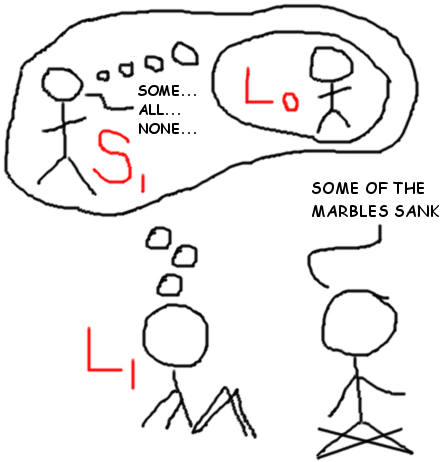
\includegraphics[scale=.8]{pics/recursivereasoning.png}
  
\end{textblock} 

\begin{textblock}{2.5}(12.3,7.4)
\red{\textbf{States of the world}}\\
$S = \{s_i | 0 \leq i \leq 15\}$% s_0, s_1, s_2, \dots, s_{15}\}$
, where $i$ indicates the number of \emph{X} that \emph{Yed}

\red{\textbf{Utterances}}\\
$\denote{u_{\textrm{none}}}= \{s_i | i = 0\}$\\  
$\denote{u_{\textrm{some}}}= \{s_i | i > 0\}$\\
$\denote{u_{\textrm{all}}}= \{s_i | i = 15\}$
  
\end{textblock} 

\begin{textblock}{3.1}(7.68,3.7)
  \begin{center}
   \mbox{\colorbox{MyGray}{
         \begin{minipage}{1.0\textwidth}
         \gray{--------------------------------------------------------------------------}
	\vspace{5cm}
         \end{minipage}
      }
   }
\end{center}
\end{textblock} 
  
%\begin{textblock}{3}(10.5,4)  
\begin{textblock}{3}(7.7,4)  
\white{\textbf{Regular RSA}}
\begin{eqnarray*} 
&&\white{P_{L_0}(s|u)\propto \delta_{\denote{u}(s)} \cdot P(s)}\\
&&\white{P_{S_1}(u|s) \propto \mathrm{exp}({\lambda \ln P_{L_0}(s|u))}}\\ 
&&\white{P_{L_1}(s|u)\propto P_{S_1}(u|s)\cdot P(s)}
\end{eqnarray*}
\end{textblock}

\begin{textblock}{4.3}(7.68,6)
  \begin{center}
   \mbox{\colorbox{MyGray}{
         \begin{minipage}{1.0\textwidth}
         \gray{--------------------------------------------------------------------------}
	\vspace{9cm}
         \end{minipage}
      }
   }
\end{center}
\end{textblock} 


\begin{textblock}{4.2}(7.7,6.3)
\white{\textbf{Wonky RSA (wRSA)}}
\begin{eqnarray*}
&&\white{P_{L_0}(s|u,w)\propto \denote{u}(s) \cdot P(s|w)}\\
&&\white{P_{S_1}(u|s,w) \propto \mathrm{exp}({\lambda \ln P_{L_0}(s|u,w))}}\\
&&\white{P_{L_1}(s,w|u)\propto P_{S_1}(u|s,w)\cdot P(s|w) \cdot P(w)}
\end{eqnarray*}
$$
\white{P(s|w) \propto \begin{cases}
1  & \text{if } w\\
   P_{\text{usual}}(s) & \text{if not } w
  \end{cases}}
  $$
  
\large

If world is wonky, use uniform prior, else use `usual' prior. Probability of wonkiness increases with unexpectedness of utterance.
  
\end{textblock}


\end{textblock}

\end{textblock}

%%%%%%%%%%%%%%%%%%%%%%%%%%%%%%%%%%%%%%%
% QUESTIONS
%%%%%%%%%%%%%%%%%%%%%%%%%%%%%%%%%%%%%%%

%\begin{textblock}{7.54}(7.4,4.7)
%  \begin{center}
%   \mbox{\colorbox{superlightgray}{
%         \begin{minipage}{1.0\textwidth}
%         \superlightgray{--------------------------------------------------------------------------}
%	\vspace{10cm}
%         \end{minipage}
%      }
%   }
%\end{center}
%
%\end{textblock} 



%%%%%%%%%%%%%%%%%%%%%%%%%%%%%%%%%%%%%%%%
%% TESTING HYPOTHESIS 1
%%%%%%%%%%%%%%%%%%%%%%%%%%%%%%%%%%%%%%%%
%
%\begin{textblock}{7.54}(7.4,12)
%  \begin{center}
%   \mbox{\colorbox{xxlightgray}{
%         \begin{minipage}{1.0\textwidth}
%         \xxlightgray{--------------------------------------------------------------------------}
%	\vspace{36cm}
%         \end{minipage}
%      }
%   }
%\end{center}
%
%\end{textblock} 
%\begin{textblock}{7.5}(7.5,12.4)
%  \LHead{Study 1: parallel pressures}
%  
%  \large
%
%\begin{textblock}{7.14}(7.6,12.6)
%  \begin{center}
%   \mbox{\colorbox{white}{
%         \begin{minipage}{1.0\textwidth}
%         \white{--------------------------------------------------------------------------}
%	\vspace{4.2cm}
%         \end{minipage}
%      }
%   }
%\end{center}
%\end{textblock} 

%\begin{textblock}{7.1}(7.7,8.7)
%
%\textbf{Dataset} 1237 cases of \emph{some}-NPs (269 partitives, 23\%) from Switchboard corpus after excluding cases that can only occur in one of the two forms (pronouns, singular count nouns, idioms)
%
%\end{textblock}
%
%\begin{textblock}{7.14}(7.6,9.8)
%  \begin{center}
%   \mbox{\colorbox{white}{
%         \begin{minipage}{1.0\textwidth}
%         \white{--------------------------------------------------------------------------}
%	\vspace{14cm}
%         \end{minipage}
%      }
%   }
%\end{center}
%\end{textblock}
%
%\begin{textblock}{7.1}(7.7,10.3)
%
%\textbf{Predictors} entered in mixed-effects logit model predicting partitive use:
%
%\vspace{.5cm}
%
%\begin{tabular}{p{10.5cm} l l}
%\toprule
%\centering \textbf{Meaning} (discourse & \multicolumn{2}{c}{\textbf{Production pressures}}\\
%\centering accessibility, \small \citeNP{reed1991}) & \multicolumn{1}{c}{Availability} & \multicolumn{1}{c}{UID} \tabularnewline
%\midrule
%\red{- previous mention of NP} & \blue{- frequency of head} & \green{- I(\normalsize{SOME}\large |  NP head)} \\
%\red{- topicality of \emph{some}-NP} & \blue{- animacy of head} & \green{- I(\normalsize{SOME}\large |  previous word)} \\
%\red{- modification of head} & \multicolumn{2}{c}{\multirow{2}{*}{Alex $\underbrace{\textrm{ate}}_{\textrm{\green{previous word}}}$ some (of the) $\underbrace{\textrm{cashews}}_{\textrm{\green{NP head}}}$}} \\
%\red{- head type (mass/count)} \\
%\bottomrule
%\end{tabular}
%
%\vspace{.4cm}
%
%I(\normalsize{SOME} \large | context) = $- \log (p(\textrm{\emph{some | }}  \textrm{context}) +  p(\textrm{\emph{some of DT | }}  \textrm{context}))$
%
%\end{textblock}


%\begin{textblock}{7.14}(7.6,13.95)
%  \begin{center}
%   \mbox{\colorbox{white}{
%         \begin{minipage}{1.0\textwidth}
%         \white{--------------------------------------------------------------------------}
%	\vspace{12cm}
%         \end{minipage}
%      }
%   }
%\end{center}
%\end{textblock}



%\begin{textblock}{4.1}(7.6,14.4)
%%\includegraphics[width=\textwidth]{pics/coefficients}
%\end{textblock}
%
%\begin{textblock}{3}(11.8,14.4)
%\red{Meaning} factors are strongest, but both \green{UID} factors and one  \blue{availability} factor affect partitive choice in  predicted direction: more partitives with increasing information of \normalsize SOME \large and decreasing availability of head.
%\end{textblock}
%
%\begin{textblock}{7.1}(7.7,14.35)
%\textbf{Results}
%\end{textblock}
%
%\end{textblock}

%%%%%%%%%%%%%%%%%%%%%%%%%%%%%%%%%%%%%%%
% PREDICTIONS AND RESULTS
%%%%%%%%%%%%%%%%%%%%%%%%%%%%%%%%%%%%%%%

\begin{textblock}{7.2}(-0.1,10.55)
%\begin{textblock}{7.54}(7.4,10.55)
  \begin{center}
   \mbox{\colorbox{superlightgray}{
         \begin{minipage}{1.0\textwidth}
         \superlightgray{--------------------------------------------------------------------------}
	\vspace{44.4cm}
         \end{minipage}
      }
   }
\end{center}
\end{textblock} 

%\begin{textblock}{2.65}(7.5,10.4)
%  \begin{center}
%   \mbox{\colorbox{superlightgray}{
%         \begin{minipage}{1.0\textwidth}
%         \superlightgray{--------------------------------------------------------------------------}
%	\vspace{23.95cm}
%         \end{minipage}
%      }
%   }
%\end{center}
%\end{textblock} 
%\begin{textblock}{7.5}(7.6,3)
\begin{textblock}{7}(0.1,11)
  \LHead{Experiments}
  
\begin{textblock}{3.3}(0.1,11.4)
  \begin{center}
   \mbox{\colorbox{white}{
         \begin{minipage}{1.0\textwidth}
         \white{--------------------------------------------------------------------------}
	\vspace{9.3cm}
         \end{minipage}
      }
   }
\end{center}

\vspace{-.7em}

  \begin{center}
   \mbox{\colorbox{white}{
         \begin{minipage}{1.0\textwidth}
         \white{--------------------------------------------------------------------------}
	\vspace{13cm}
         \end{minipage}
      }
   }
\end{center}

\vspace{-.7em}

  \begin{center}
   \mbox{\colorbox{white}{
         \begin{minipage}{1.0\textwidth}
         \white{--------------------------------------------------------------------------}
	\vspace{12.6cm}
         \end{minipage}
      }
   }
\end{center}
  
\end{textblock} 

\begin{textblock}{3.2}(0.2,11.8)
\large
%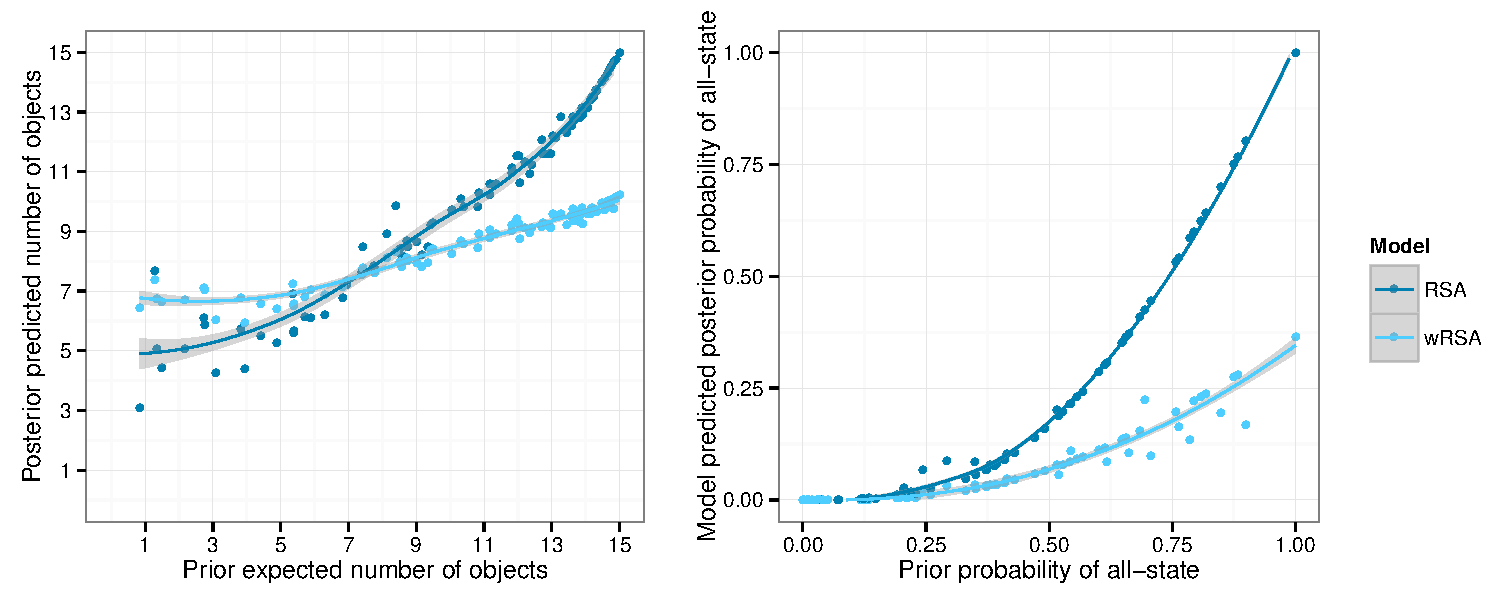
\includegraphics[width=\textwidth]{pics/rsa-predictions}
%\emph{John threw 15 marbles into a pool.}

\textbf{\red{Experiment 1: prior elicitation}}

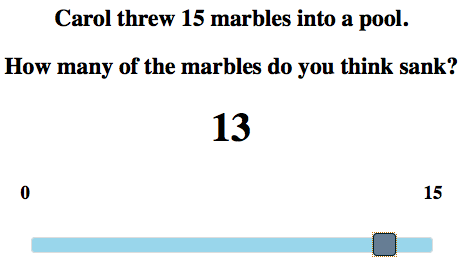
\includegraphics[width=\textwidth]{pics/display-priors.png}

\vspace{.6em}

\textbf{\red{Experiment 2a: comprehension\\(expected number of objects)}}

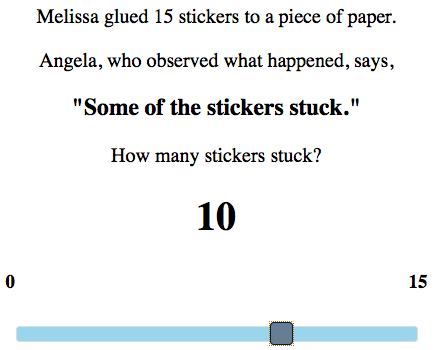
\includegraphics[width=1.05\textwidth]{pics/display-priordv.png}

\vspace{.6em}

\textbf{\red{Experiment 2b: comprehension\\(posterior all-state probability)}}

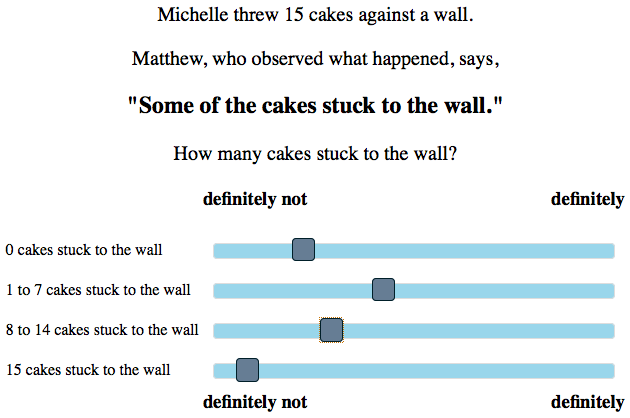
\includegraphics[width=1.05\textwidth]{pics/display-allprob.png}


\end{textblock} 
  


\begin{textblock}{3.1}(3.8,12)

\begin{textblock}{3.25}(3.7,11.4)
  \begin{center}
   \mbox{\colorbox{white}{
         \begin{minipage}{1.0\textwidth}
         \white{--------------------------------------------------------------------------}
	\vspace{9.3cm}
         \end{minipage}
      }
   }
\end{center}

\vspace{-.7em}

  \begin{center}
   \mbox{\colorbox{white}{
         \begin{minipage}{1.0\textwidth}
         \white{--------------------------------------------------------------------------}
	\vspace{16.5cm}
         \end{minipage}
      }
   }
\end{center}

\vspace{-.7em}
  \begin{center}
   \mbox{\colorbox{white}{
         \begin{minipage}{1.0\textwidth}
         \white{--------------------------------------------------------------------------}
	\vspace{9.1cm}
         \end{minipage}
      }
   }
\end{center}

\end{textblock}

\large

\vspace{-1.2em}

\textbf{Overview}\\
1. Estimate prior beliefs about how many X Y (Exp.~1)\\
2. Estimate listeners' posterior beliefs about how many X Yed (Exp.~2a and 2b) and how likely the world is wonky (Exp.~3) to test RSA and wRSA models
%\hspace{2cm} How many X Yed (Exp.~2a)?\\
%\hspace{2cm} How likely is it that all X Yed (Exp.~2b)?\\
%\hspace{2cm} How wonky (normal) are the objects involved in the event?

\vspace{.25em}
\textbf{Experimental details}\\
90 items: \textbf{\emph{Q of the X Yed}}\\
 \emph{Q}: \emph{some} (10), \emph{all} (5), \emph{none} (5)\\
 \emph{X}: \emph{marbles, shirts, carrots,\dots}\\
 \emph{Y}: \emph{sank, ripped, dissolved,\dots}
 
% \vspace{.1em}
30 trials per participant in each experiment, including 5 short \\fillers (\emph{Typical}) and 5 long fillers (\emph{What a stupid thing to do.})

Participants in each experiment

\normalsize
\begin{tabular}{l c c c c}
\toprule
 & Exp.~1 & Exp.~2a & Exp.~2b & Exp.~3 \\
\midrule
\textbf{n} & 60 & 120 & 120 & 60\\
\bottomrule
\end{tabular}

\vspace{1.2em}

\large

\textbf{\red{Experiment 3: wonkiness}}

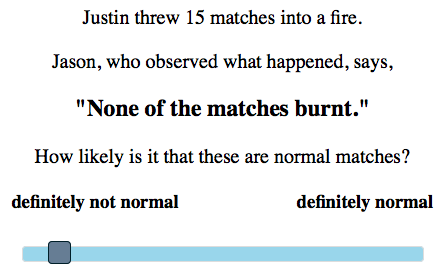
\includegraphics[width=\textwidth]{pics/display-wonky.png}


\end{textblock} 

%
%\begin{textblock}{7.04}(7.7,16.1)
%\hspace{4cm} \red{\textbf{Experiment 2a}} \hspace{8cm} \red{\textbf{Experiment 2b}}\\
%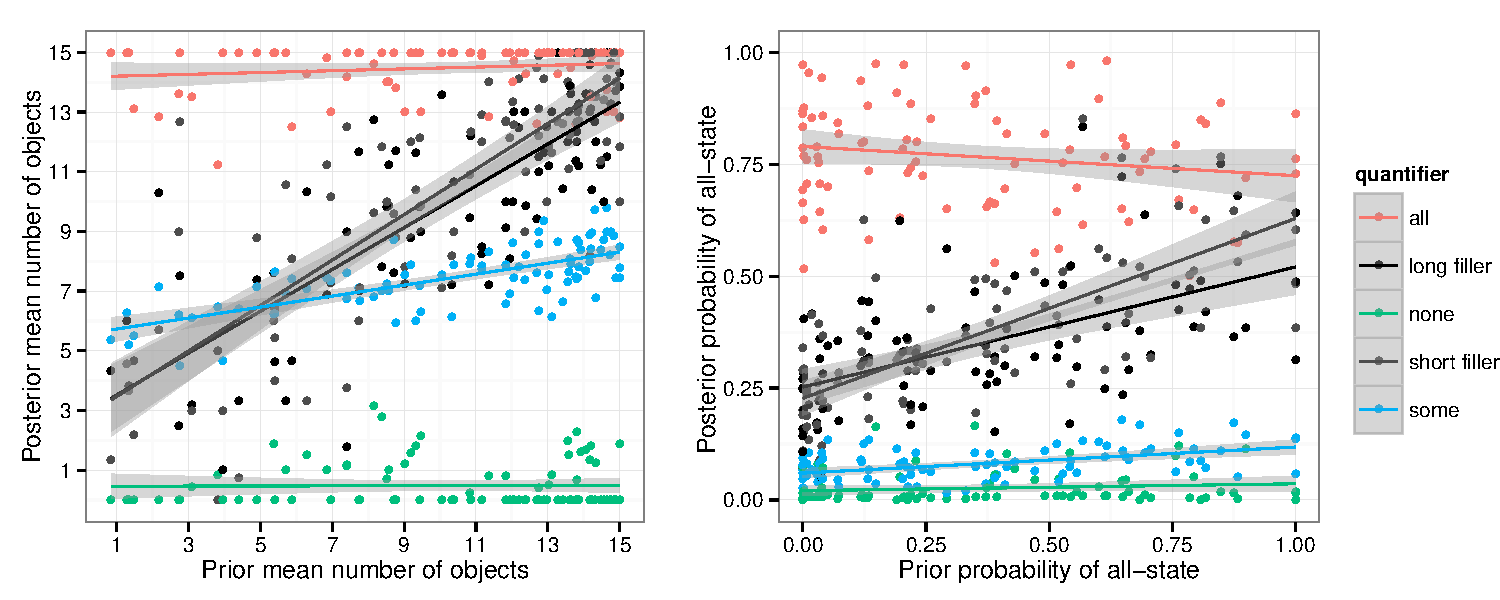
\includegraphics[width=\textwidth]{pics/empirical-results}
%\end{textblock} 
%
\end{textblock} 

%%%%%%%%%%%%%%%%%%%%%%%%%%%%%%%%%%%%%%%
% CONCLUSION
%%%%%%%%%%%%%%%%%%%%%%%%%%%%%%%%%%%%%%%

\begin{textblock}{7.2}(-0.1,22.9)
  \begin{center}
   \mbox{\colorbox{xxlightgray}{
         \begin{minipage}{1.0\textwidth}
         \superlightgray{--------------------------------------------------------------------------}
	\vspace{11.6cm}
         \end{minipage}
      }
   }
\end{center}

\end{textblock} 

\begin{textblock}{7}(0.1,23.3)
\LHead{Conclusion}

\large
The effect of  world knowledge (prior beliefs) on interpretation was much smaller, and qualitatively different, than predicted by a standard Bayesian model of quantifier interpretation (RSA). Extending RSA with a lifted wonkiness variable that captures whether listeners think the world is wonky upon encountering an odd utterance, and allows them to back off to alternative beliefs, provided a good fit to the data, suggesting: \textbf{listeners revise common ground when utterances are odd}. % empirical wonkiness judgments and improved the fit to participants' comprehension data. %This is the first attempt to explicitly model the quantitative effect of world knowledge and its defeasibility on pragmatic utterance interpretation.


\end{textblock} 

%\begin{textblock}{7}(0.1,11)
%  \LHead{Experiments}
%  
%\begin{textblock}{6.8}(0.1,11.4)
%  \begin{center}
%   \mbox{\colorbox{white}{
%         \begin{minipage}{1.0\textwidth}
%         \white{--------------------------------------------------------------------------}
%	\vspace{40.5cm}
%         \end{minipage}
%      }
%   }
%\end{center}
%
%  
%\end{textblock} 
%
%\begin{textblock}{6.7}(0.2,11.7)
%bla
%\end{textblock}


%%%%%%%%%%%%%%%%%%%%%%%%%%%%%%%%%%%%%%%
% PREDICTIONS AND RESULTS
%%%%%%%%%%%%%%%%%%%%%%%%%%%%%%%%%%%%%%%

%\begin{textblock}{7.2}(-0.1,12.97)
\begin{textblock}{7.54}(7.4,10.55)
  \begin{center}
   \mbox{\colorbox{xxlightgray}{
         \begin{minipage}{1.0\textwidth}
         \superlightgray{--------------------------------------------------------------------------}
	\vspace{53cm}
         \end{minipage}
      }
   }
\end{center}
\end{textblock} 

%\begin{textblock}{2.65}(7.5,10.4)
%  \begin{center}
%   \mbox{\colorbox{superlightgray}{
%         \begin{minipage}{1.0\textwidth}
%         \superlightgray{--------------------------------------------------------------------------}
%	\vspace{23.95cm}
%         \end{minipage}
%      }
%   }
%\end{center}
%\end{textblock} 
%\begin{textblock}{7.5}(7.6,3)
\begin{textblock}{7.44}(7.6,11)
  \LHead{\hspace{1em} Empirical results \hspace{3.2em} Model predictions}
  
\begin{textblock}{7.1}(7.6,11.4)
  \begin{center}
   \mbox{\colorbox{white}{
         \begin{minipage}{1.0\textwidth}
         \white{--------------------------------------------------------------------------}
	\vspace{33cm}
         \end{minipage}
      }
   }
\end{center}


%  \begin{center}
%   \mbox{\colorbox{white}{
%         \begin{minipage}{1.0\textwidth}
%         \white{--------------------------------------------------------------------------}
%	\vspace{16cm}
%         \end{minipage}
%      }
%   }
%\end{center}

  \begin{center}
   \mbox{\colorbox{white}{
         \begin{minipage}{1.0\textwidth}
         \white{--------------------------------------------------------------------------}
	\vspace{14.5cm}
         \end{minipage}
      }
   }
\end{center}
  
\end{textblock} 

\begin{textblock}{7.04}(7.7,11.7)

\begin{center}
%\LHead{Interpretation}
\large
\textbf{Comprehension}

\vspace{-0.5em}

\textbf{\red{Experiment 2a}} \hspace{9em} \textbf{\red{$\mathbb{E}[P(s|u_{\textrm{some}})]$}}\\
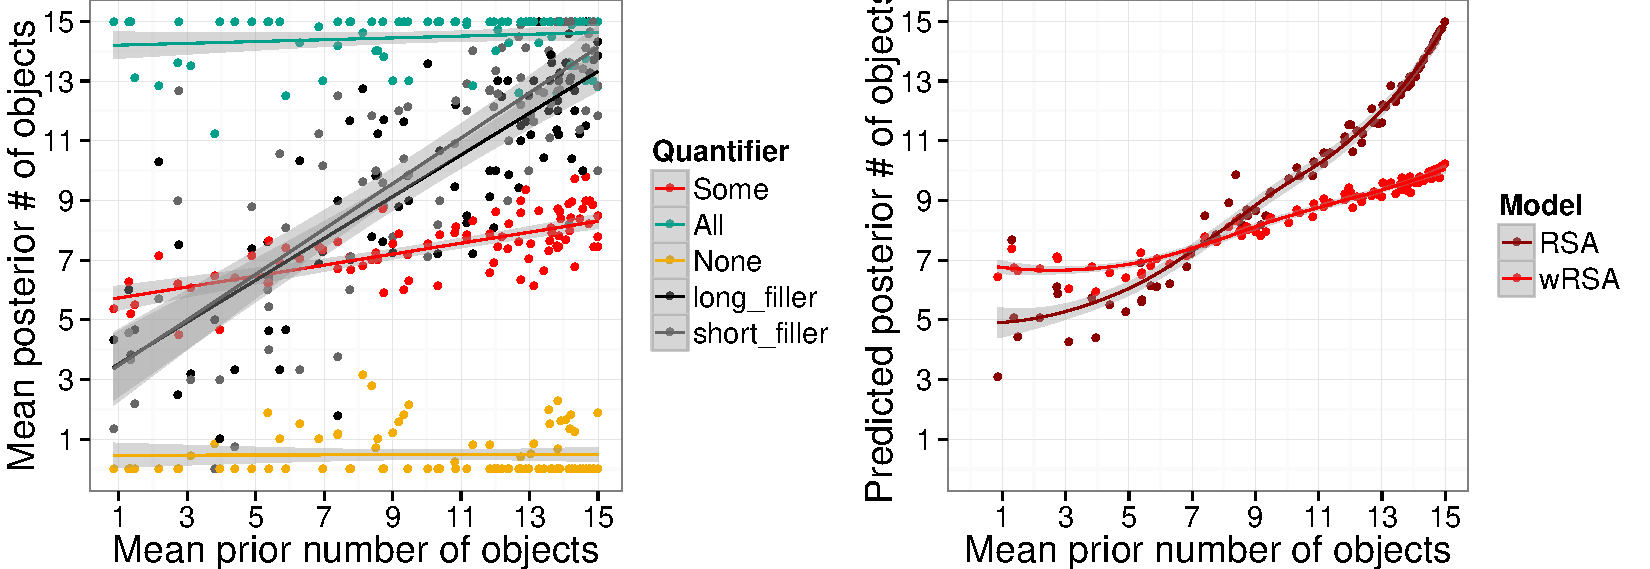
\includegraphics[width=1.01\textwidth]{pics/model-empirical-expectations}

%\vspace{1em}

\hspace{-1em} \textbf{\red{Experiment 2b}} \hspace{9em} \textbf{\red{$P(s_{15}|u_{\textrm{some}})$}}\\
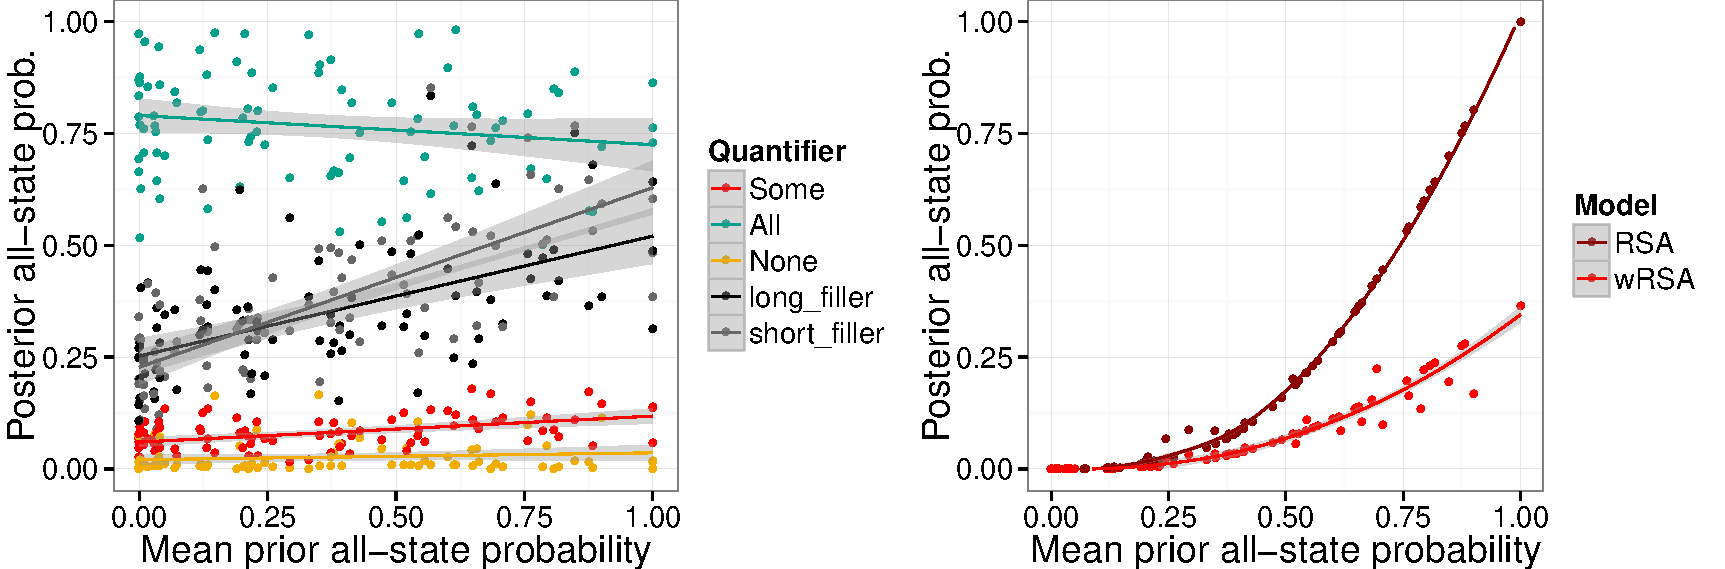
\includegraphics[width=1.01\textwidth]{pics/model-empirical-allprobs}

\end{center}

\large
Robust effect of prior on posterior expectation ($\beta$=.18, $SE$=.02, $t$=7.4, $p$$<$.0001) and all-state probability ($\beta$=.06, $SE$=.01, $t$=5.0, $p$$<$.0001). But: effect is much smaller than predicted by RSA. The data are much better fit by the wonky RSA model.

\vspace{1.5em}

\begin{center}
\large
\textbf{Wonkiness}

\vspace{-0.5em}

\hspace{-1.5em} \textbf{\red{Experiment 3}} \hspace{8.5em} \textbf{\red{$P(w|u)$}}\\
\centering
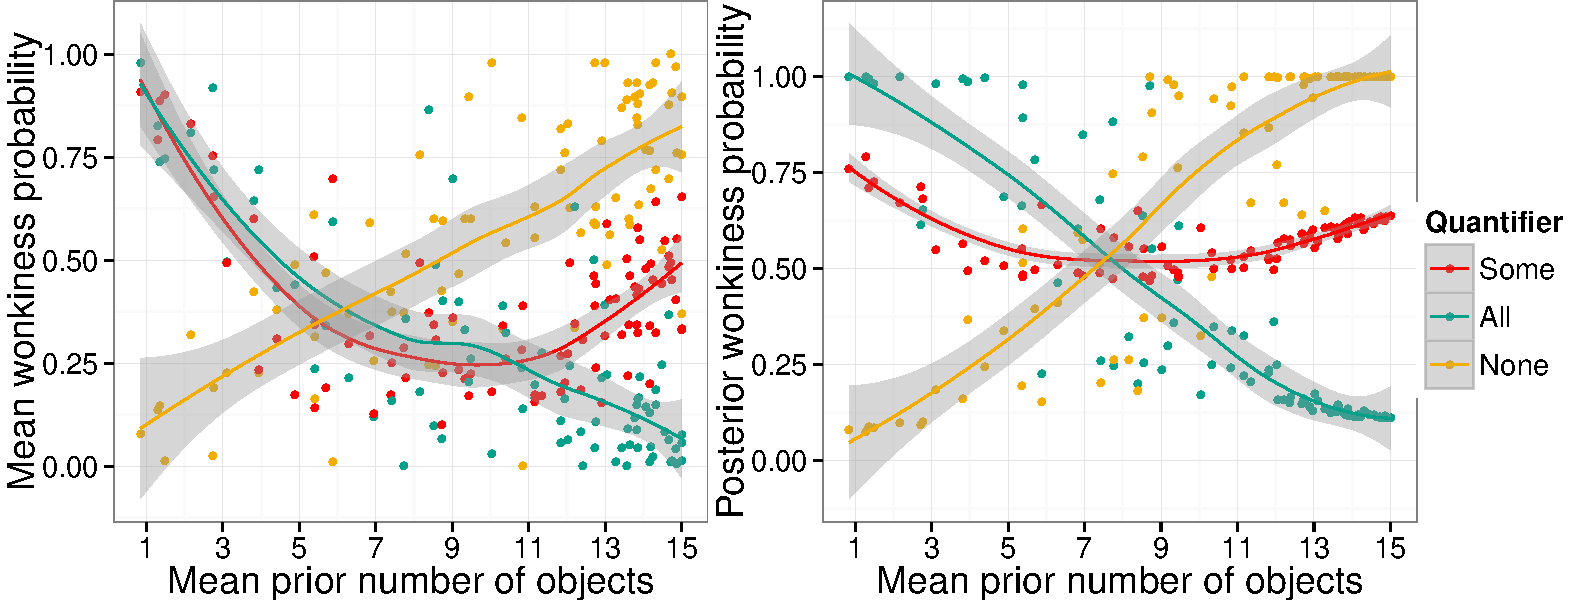
\includegraphics[width=\textwidth]{pics/model-empirical-wonkiness}
\end{center}

\end{textblock} 

\end{textblock} 

%%%%%%%%%%%%%%%%%%%%%%%%%%%%%%%%%%%%%%%%
%% PREDICTIONS AND RESULTS FOR WONKINESS
%%%%%%%%%%%%%%%%%%%%%%%%%%%%%%%%%%%%%%%%
%
%%\begin{textblock}{7.2}(-0.1,12.97)
%\begin{textblock}{7.54}(7.4,21)
%  \begin{center}
%   \mbox{\colorbox{superlightgray}{
%         \begin{minipage}{1.0\textwidth}
%         \superlightgray{--------------------------------------------------------------------------}
%	\vspace{18cm}
%         \end{minipage}
%      }
%   }
%\end{center}
%\end{textblock} 
%
%%\begin{textblock}{2.65}(7.5,10.4)
%%  \begin{center}
%%   \mbox{\colorbox{superlightgray}{
%%         \begin{minipage}{1.0\textwidth}
%%         \superlightgray{--------------------------------------------------------------------------}
%%	\vspace{23.95cm}
%%         \end{minipage}
%%      }
%%   }
%%\end{center}
%%\end{textblock} 
%%\begin{textblock}{7.5}(7.6,3)
%\begin{textblock}{7.44}(7.6,21.5)
%  \LHead{Wonkiness: model predictions and empirical results}
%  
%\begin{textblock}{7.1}(7.6,21.8)
%  \begin{center}
%   \mbox{\colorbox{white}{
%         \begin{minipage}{1.0\textwidth}
%         \white{--------------------------------------------------------------------------}
%	\vspace{14cm}
%         \end{minipage}
%      }
%   }
%\end{center}
%  
%\end{textblock} 
%
%\begin{textblock}{7.04}(7.7,22.2)
%\hspace{5.5cm} \red{\textbf{Model}} \hspace{10cm} \red{\textbf{Experiment 3 }}\\
%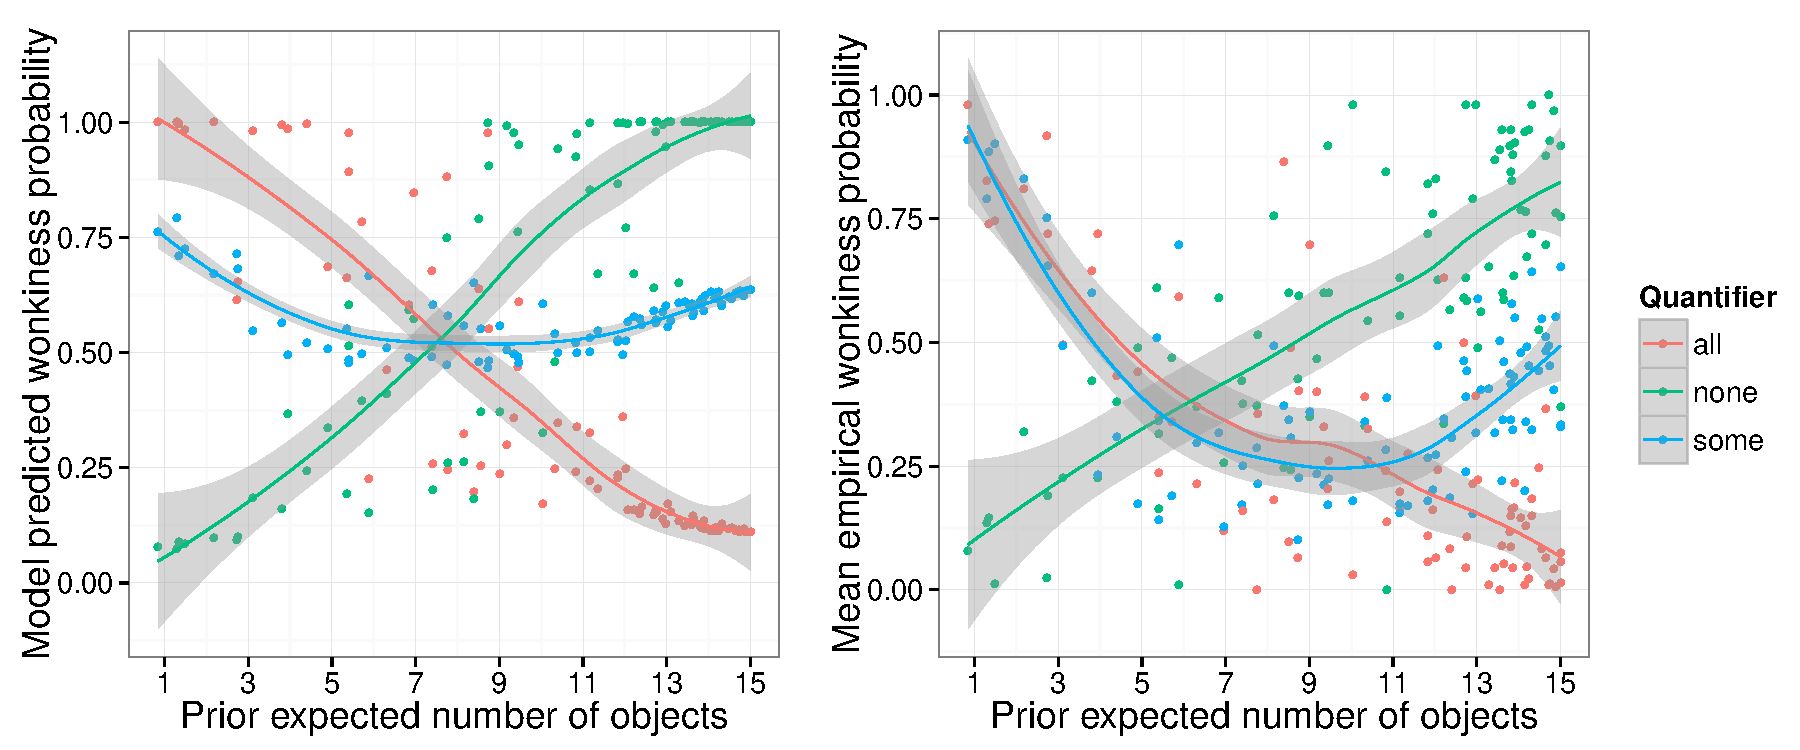
\includegraphics[width=\textwidth]{pics/wonkiness-fullplot}
%\end{textblock} 
%
%\end{textblock} 


%%%%%%%%%%%%%%%%%%%%%%%%%%%%%%%%%%%%%%%
% REFERENCES AND ACKNOWLEDGMENTS
%%%%%%%%%%%%%%%%%%%%%%%%%%%%%%%%%%%%%%%
\begin{textblock}{7}(7.4,25.3)
\small
\textbf{Acknowledgments}
This work was supported by a James S. McDonnell Foundation Scholar Award and and ONR grant N00014-13-1-0287 (NDG).
\end{textblock}


\renewcommand{\refname}{\normalsize References}

\begin{textblock}{7}(7.4,25.75)
\small
\textbf{References}
\end{textblock}

\renewcommand{\refname}{}
\begin{textblock}{6}(8.3,24.95)
\let\bibliographytypesize\scriptsize\bibliographystyle{apacitex}
\bibliographystyle{apacitex}
\bibliography{bibs}  
\end{textblock}

%\begin{textblock}{8.66}(6.44,22.9)
%  \begin{center}
%   \mbox{\colorbox{white}{
%         \begin{minipage}{1.0\textwidth}
%         \white{--------------------------------------------------------------------------}
%	\vspace{8.5cm}
%         \end{minipage}
%      }
%   }
%\end{center}

%\end{textblock} 

%\begin{textblock}{8.7}(6.42,22.88)
%  \begin{center}
%   \mbox{\colorbox{MyGray}{
%         \begin{minipage}{1.0\textwidth}
%         \white{--------------------------------------------------------------------------}
%	\vspace{8.7cm}
%         \end{minipage}
%      }
%   }
%\end{center}

%\end{textblock} 

\end{document}

